%&pdflatex
\documentclass[11pt, a4paper]{article}
\usepackage{graphicx}
\usepackage{amsmath}
\usepackage{listings}
\usepackage{minted}
\usepackage{physics}
\usepackage{hyperref}
\hypersetup{
    colorlinks=true, %set true if you want colored links
    linktoc=all,     %set to all if you want both sections and subsections linked
    linkcolor=magenta,  %choose some color if you want links to stand out
}

\title{EE2703 Applied Programming Lab - Assignment No 9}
\author{
  \textbf{Name}: Abishek S\\
  \textbf{Roll Number}: EE18B001
}\date{\today}
\begin{document}
		
\maketitle 
\section{Abstract}
The goal of the assignment is the following :
\begin{itemize}
\item Obtaining the DFT of non-periodic signals.
\item To understand the use of windowing functions (e.g. Hamming Window) to reduce the effect of Gibbs phenomenon.
\item To analyse the chirped signal.
\end{itemize}
\usemintedstyle{manni}


\section{Assignment}
\subsection{Setting up the environment}
Importing the necessary libraries
\begin{minted}[mathescape,escapeinside = ||]{python3}
from pylab import *
import sys
import mpl_toolkits.mplot3d.axes3d as p3
from matplotlib import cm
\end{minted}
Defining the DFT function (that was used in the previous assignment to generate spectrum) again for our ease
\begin{minted}{python3}
def DFT(y_fn,tim = (-4*pi,4*pi),N = 512,name = ''):
	''' Utility function for generating spectrum of given function.

	y_fn : function for which spectrum needs to be obtained
	tim : time interval of form (starting time,ending time) 
		where ending time has to be excluded
	N : number of samples in time domain
	name : Name of function for the spectrum
	'''
	st,end = tim

	t = linspace(st,end,N,endpoint = False)
	y = y_fn(t)
	#The sample corresponding to -tmax should be set zero
	y[0] = 0 
	Y = fftshift(fft(fftshift(y)))/float(N)
	w = linspace(-pi,pi,N,endpoint = False)
	#The range of frequencies
	w = w*(N/(end-st))

	fig, (ax1,ax2) = subplots(2,1)
	suptitle(f"Spectrum of {name}")
	ax1.plot(w,abs(Y),lw=1)
	ax1.set_ylabel(r"$|Y|$",size=16)
	ax1.grid(True)

	ax2.plot(w,angle(Y),'ro',lw=1)  
	ax2.grid(True)
	ax2.set_ylabel(r"Phase of $Y$",size=16)
	ax2.set_xlabel(r"$\omega$",size=16)

	return ax1,ax2,Y,w
\end{minted}


\subsection{EXAMPLE 1 - FFT of $\sin(\sqrt{2} t)$ - Trial 1}
{
We find the spectrum of $\sin(\sqrt{2} t)$ which does not cover an integral multiple of cycles in the time interval taken.
}
\begin{minted}{python3}
y1 = lambda t: sin(sqrt(2)*t)
DFT(y1,(-pi,pi),64,r"$\sin(\sqrt{2}t)$")
show()
\end{minted}

\begin{figure}[H]
   	\centering
   	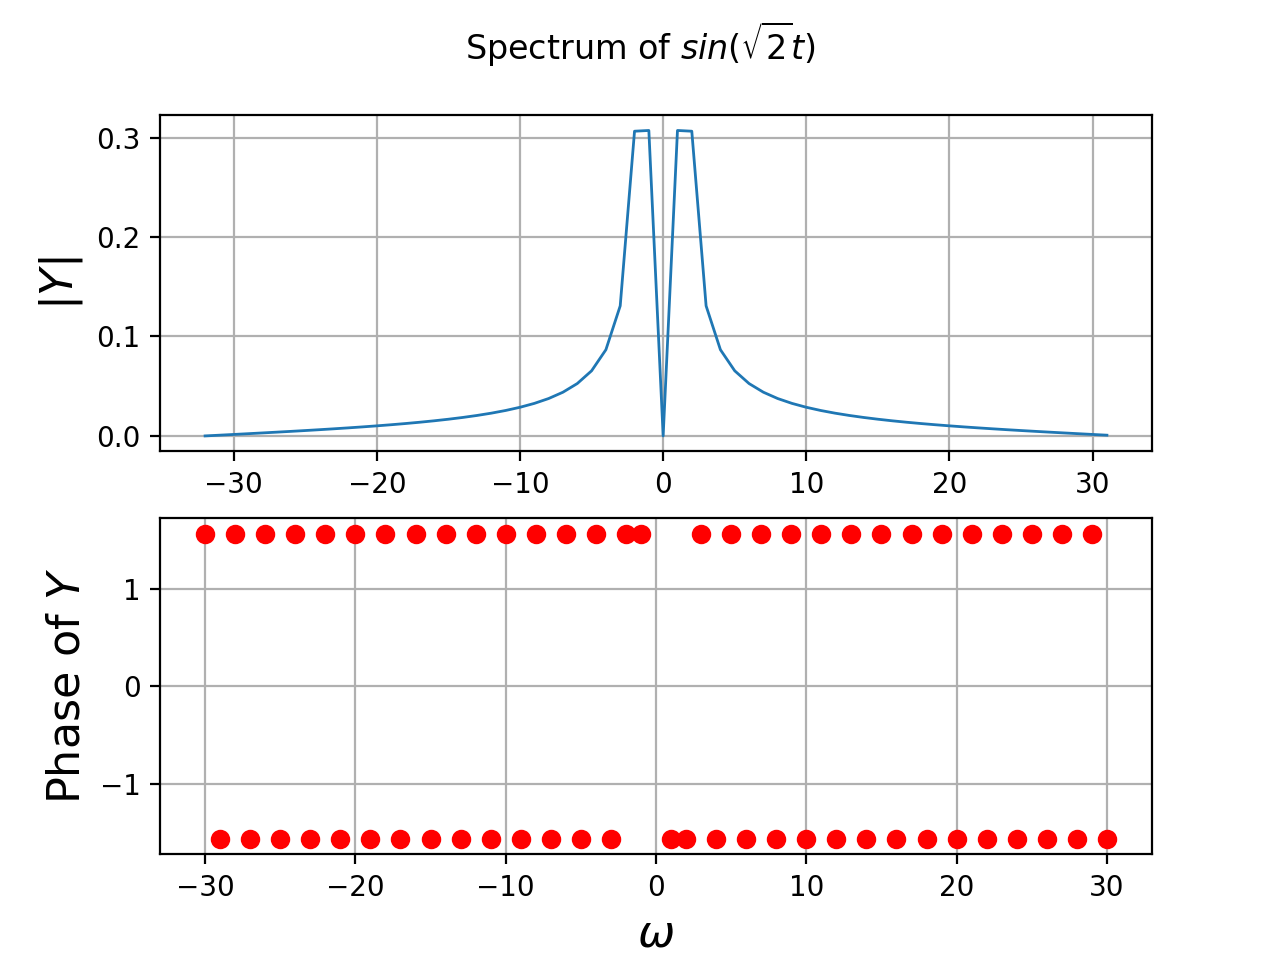
\includegraphics[scale=0.8]{ex_1_i.png}
   	\label{fig:ex_1_i}
   	\caption{DFT Spectrum of $\sin(\sqrt{2} t)$}
\end{figure}
{
Notice that we set $y[\frac{N}{2}] = 0$ so that DFT is purely imaginary.
\\We expected \textbf{two peaks} at $\pm \sqrt{2}$ but we instead \textbf{got two broad peaks with gradually decaying magnitude}. The phase is correct. 
}


\subsection{EXAMPLE 1 - Analysing above results}
{
We plot the extensions of the sinusoid function we took and also plot replications of our function taken in a specific interval in one interval each above and below our chosen time interval.
}
\begin{minted}{python3}
t1=linspace(-pi,pi,65);t1=t1[:-1]
t2=linspace(-3*pi,-pi,65);t2=t2[:-1]
t3=linspace(pi,3*pi,65);t3=t3[:-1]
# y=sin(sqrt(2)*t)
figure()
plot(t1,sin(sqrt(2)*t1),'b',lw=2)
plot(t2,sin(sqrt(2)*t2),'r',lw=2)
plot(t3,sin(sqrt(2)*t3),'r',lw=2)
ylabel(r"$y$",size=16)
xlabel(r"$t$",size=16)
title(r"$\sin\left(\sqrt{2}t\right)$")
grid(True)
show()

y=sin(sqrt(2)*t1)
figure()
plot(t1,y,'bo',lw=2)
plot(t2,y,'ro',lw=2)
plot(t3,y,'ro',lw=2)
ylabel(r"$y$",size=16)
xlabel(r"$t$",size=16)
title(r"$\sin\left(\sqrt{2}t\right)$ with $t$ wrapping every $2\pi$ ")
grid(True)
show()
\end{minted}

\begin{figure}[H]
   	\centering
   	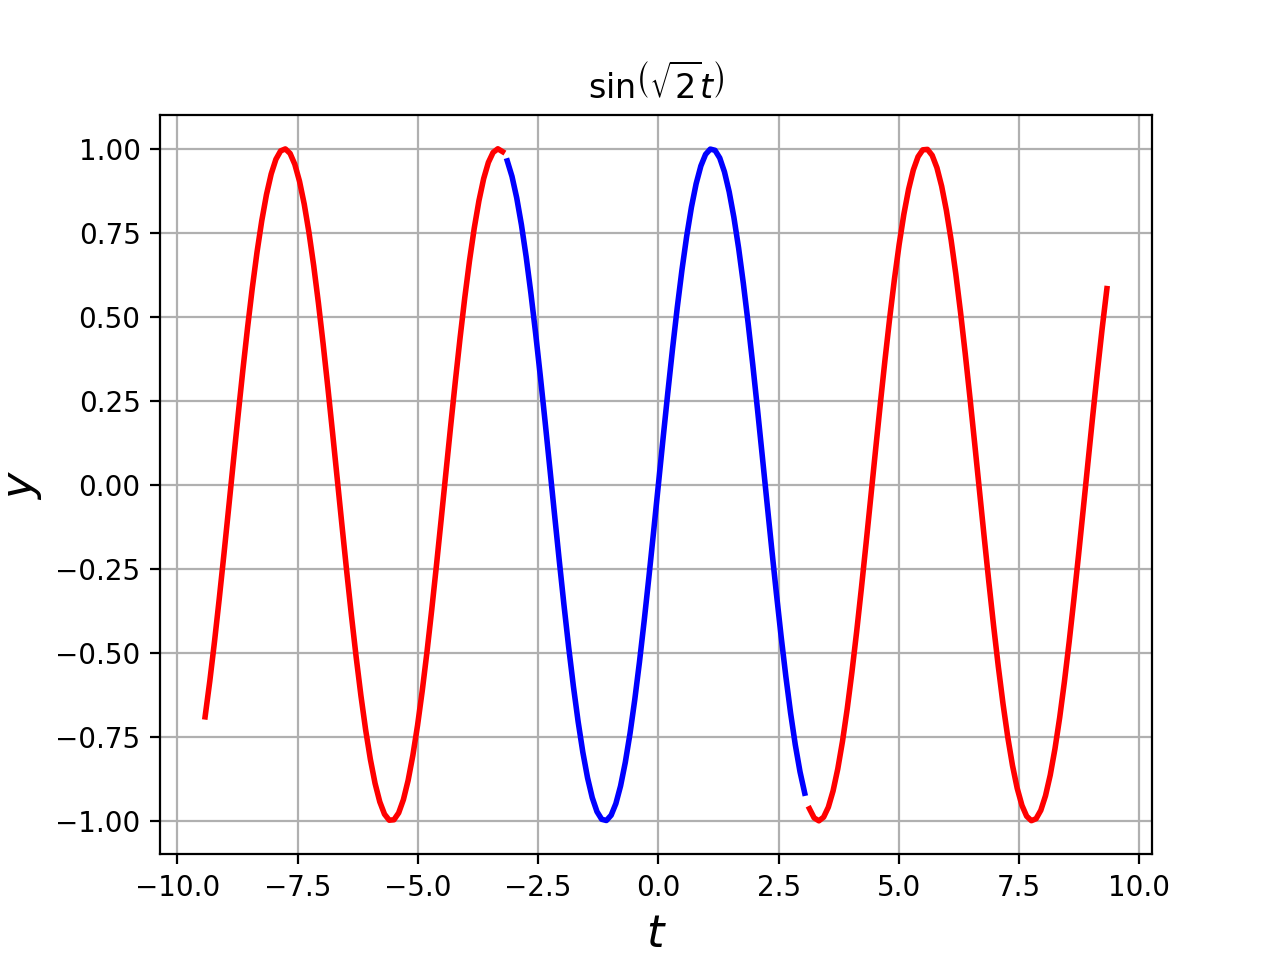
\includegraphics[scale=0.5]{ex_1_ext.png}
   	\label{fig:ex_1_ext}
   	\caption{Extensions of $\sin(\sqrt{2} t)$ function outside $[-\pi,\pi)$}
\end{figure}
\begin{figure}[H]
   	\centering
   	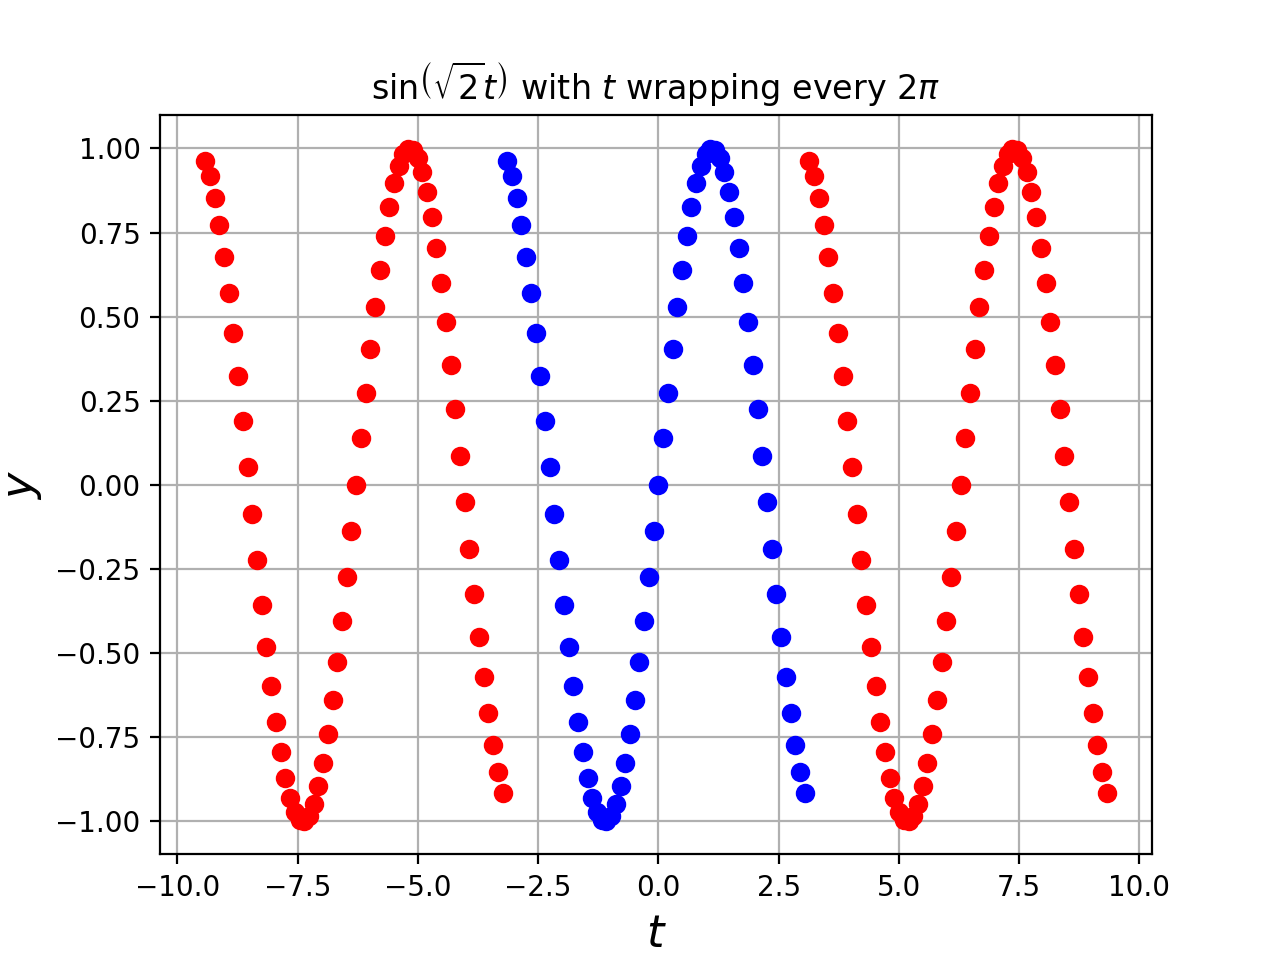
\includegraphics[scale=0.5]{ex_1_rep.png}
   	\label{fig:ex_1_rep}
   	\caption{Replications of $\sin(\sqrt{2} t)$ function outside $[-\pi,\pi)$}
\end{figure}
{
We can clearly notice that the two signals \textbf{aren't the same} and there are also \textbf{discontinuities} that appear in the replications which lead to Gibbs phenomenon, that in turn causes the slowly decaying peak.
}


\subsection{EXAMPLE 1 - Using windowing to diminish Gibbs phenomenon} 
{
We observed that the \textbf{Gibbs phenomenon is the reason for the slowly decaying peaks} of the spectrum. We can verify this for digital ramp by plotting its semilog plot.
}
\begin{minted}{python3}
t=linspace(-pi,pi,65);t=t[:-1]
dt=t[1]-t[0];fmax=1/dt
y=t
#The sample corresponding to -tmax should be set zero
y[0]=0 
y=fftshift(y) #make y start with y(t=0)
Y=fftshift(fft(y))/64.0
w=linspace(-pi*fmax,pi*fmax,65);w=w[:-1]
figure()
semilogx(abs(w),20*log10(abs(Y)),lw=2)
xlim([1,10])
ylim([-20,0])
xticks([1,2,5,10],["1","2","5","10"],size=16)
ylabel(r"$|Y|$ (dB)",size=16)
title(r"Spectrum of a digital ramp")
xlabel(r"$\omega$",size=16)
grid(True)
show()
\end{minted}

\begin{figure}[H]
   	\centering
   	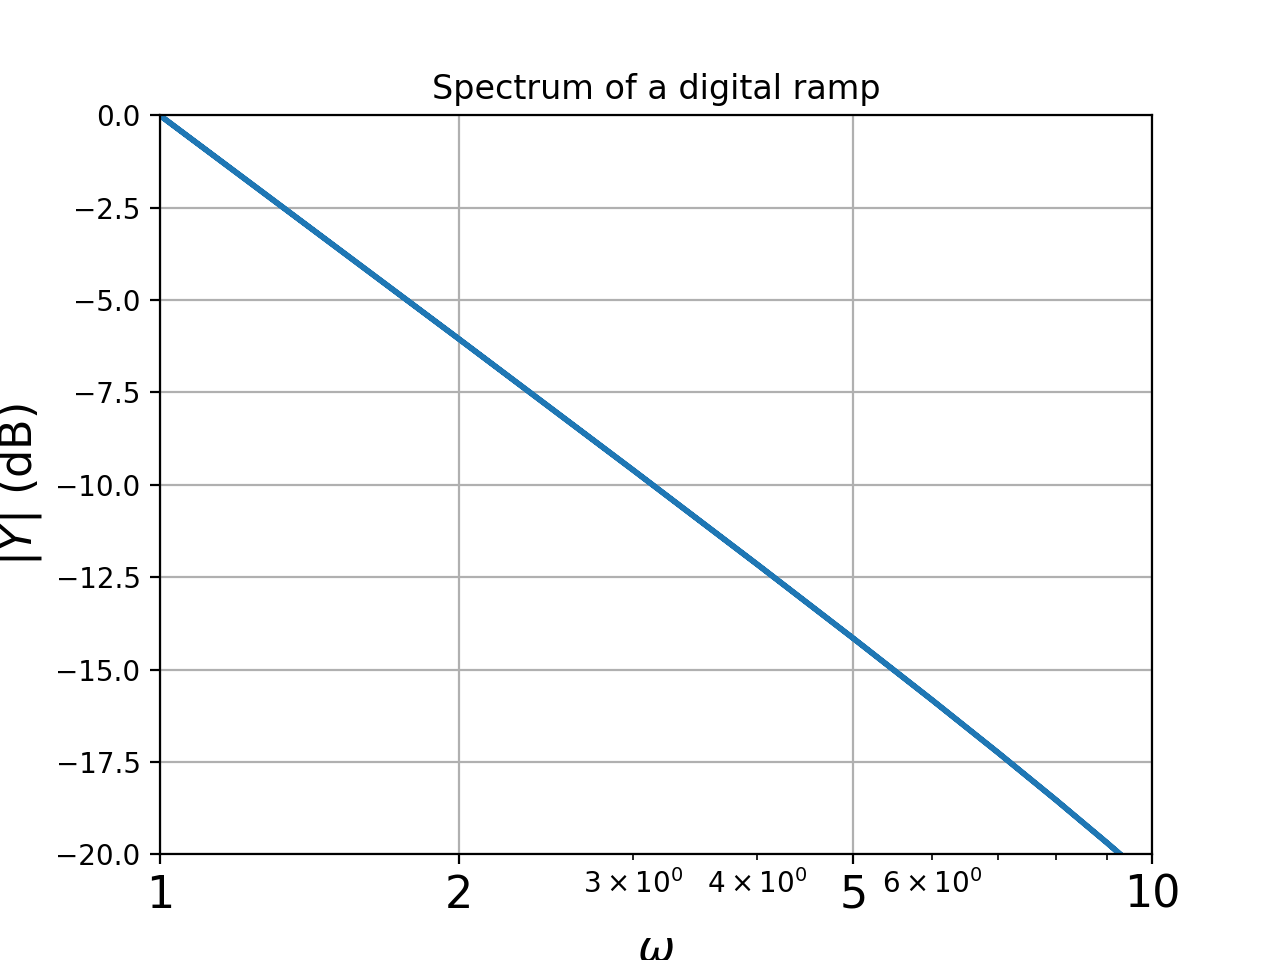
\includegraphics[scale=0.5]{ex_1_bode.png}
   	\label{fig:ex_1_bode}
   	\caption{Semilog plot of digital ramp function's spectrum}
\end{figure}
{
We can clearly see the slope is nearly -20 $\frac{dB}{dec}$ which means that the DFT amplitude falls as $\frac{1}{\omega}$.
\\We need to damp the function at the ends of the periodic interval. We do this by multiplying the original function with a windowing function (here, the Hamming window - a raised cosine function), which boosts the spectrum at the centre and suppresses at the ends.
\\Let's now plot the resulting signal obtained by multiplying  $f[n] = \sin(\sqrt{2} t)$ with the \textbf{Hamming Window} $w[n]$.
}
\begin{align*}
w[n] = \begin{cases}
 			0.54 + 0.46 \cos(\frac{2\pi n}{N-1}) & |n| \leq \frac{N-1}{2}  \\
 			 0  & else
		  \end{cases}
\end{align*}
\[
g[n] = f[n]\ w[n]
\]
\[
G_k = \sum_{n = 0}^{N - 1} F_n W_{k-n}
\]
\begin{minted}{python3}
t=linspace(-pi,pi,65);t=t[:-1]
wnd = lambda t: fftshift(0.54+0.46*cos(2*pi*t/len(t)))  #hamming window
t1=linspace(-pi,pi,65);t1=t1[:-1]
t2=linspace(-3*pi,-pi,65);t2=t2[:-1]
t3=linspace(pi,3*pi,65);t3=t3[:-1]
n=arange(64)
y=sin(sqrt(2)*t1)*wnd(n)
figure()
plot(t1,y,'bo',lw=2)
plot(t2,y,'ro',lw=2)
plot(t3,y,'ro',lw=2)
ylabel(r"$y$",size=16)
xlabel(r"$t$",size=16)
title(r"$\sin\left(\sqrt{2}t\right)\times w(t)$ with $t$ wrapping every $2\pi$")
grid(True)
show()
\end{minted}

\begin{figure}[H]
   	\centering
   	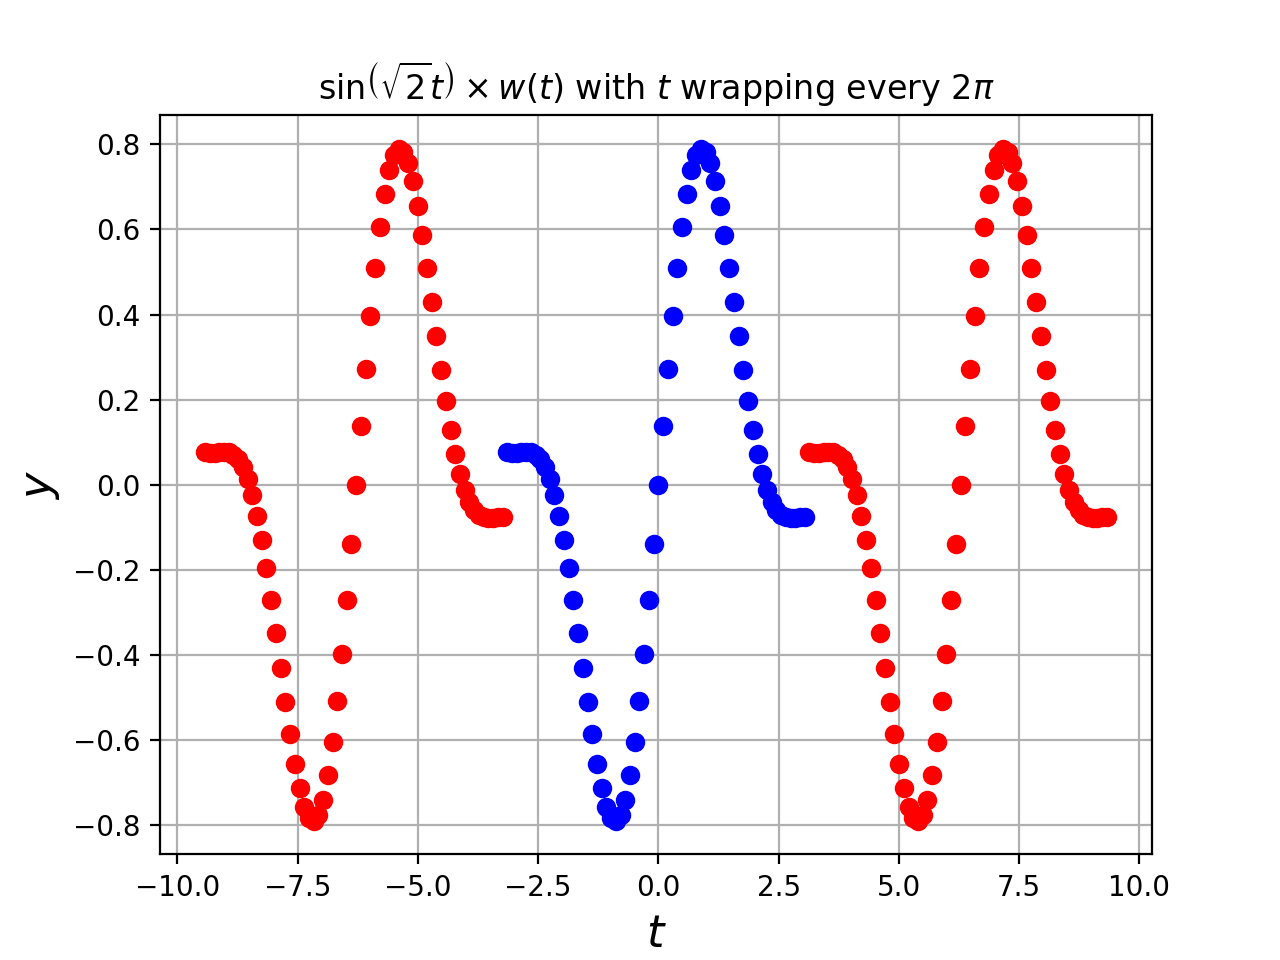
\includegraphics[scale=0.5]{ex_1_wnd.png}
   	\label{fig:ex_1_wnd}
   	\caption{Windowed $\sin(\sqrt{2} t)$ signal}
\end{figure}
{
We notice that the \textbf{discontinuities are very much reduced} now due to the windowing, still is not completely eliminated though.
}


\subsection{EXAMPLE 1 - FFT of $\sin(\sqrt{2} t)$ - Trial 2} 
{
We take the windowed $\sin(\sqrt{2} t)$  function and find the spectrum.
}
\begin{minted}{python3}
y2 = lambda t,n: sin(sqrt(2)*t)*wnd(arange(n))
y2_64 = lambda t : y2(t,64)
ax1,ax2,*_ = DFT(y2_64,(-pi,pi),64,r'$\sin(\sqrt{2}t*w(n)$)')
ax1.set_xlim(-8,8)
ax2.set_xlim(-8,8)
show()
\end{minted}

\begin{figure}[H]
   	\centering
   	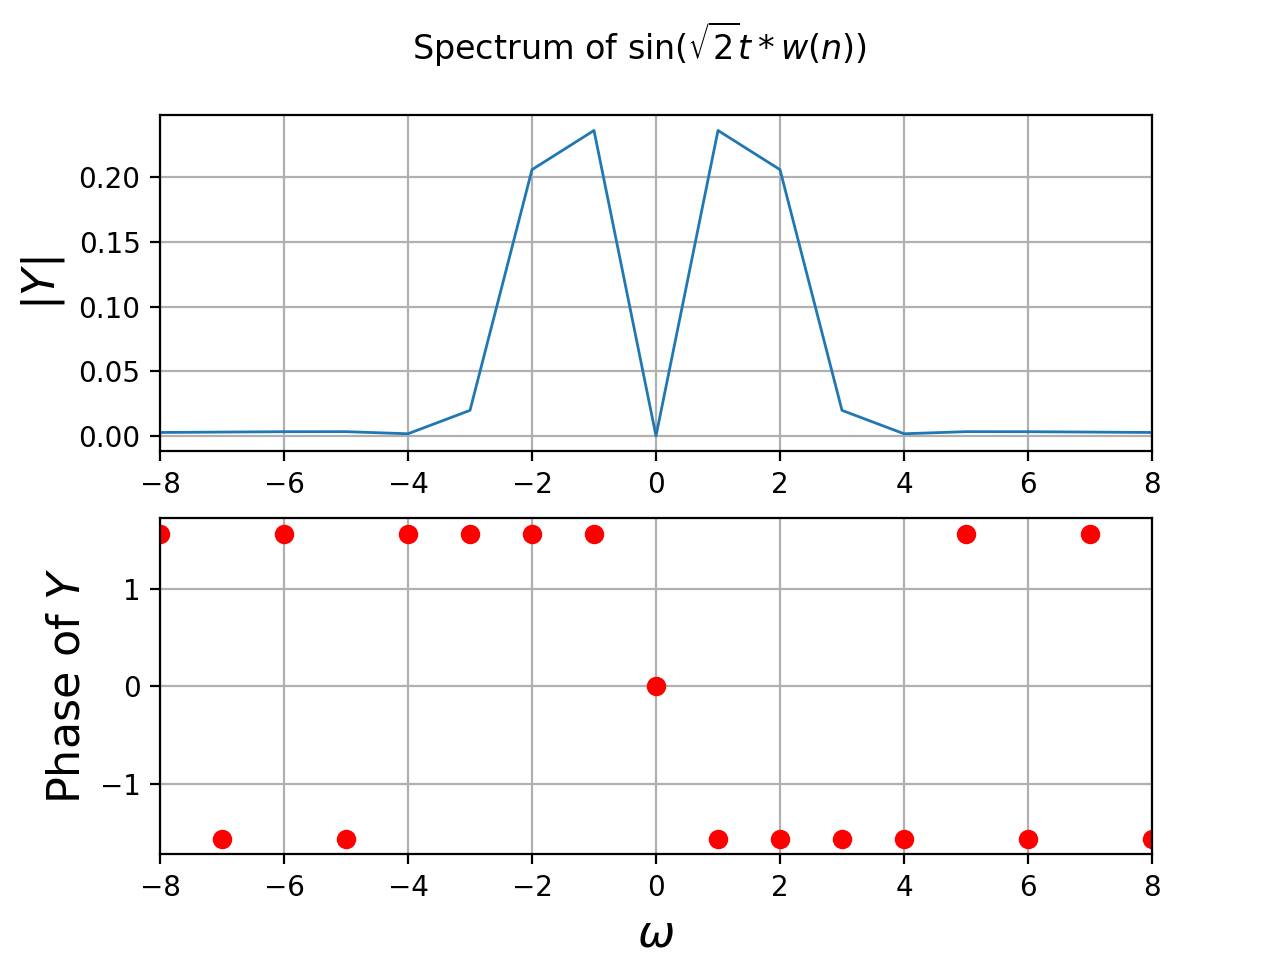
\includegraphics[scale=0.8]{ex_1_f.png}
   	\label{fig:ex_1_f}
   	\caption{Spectrum of $\sin(\sqrt{2} t)$ - obtained with 64 samples}
\end{figure}
{
The spectrum is now much better. The peaks still are \textbf{two samples wide} since $\sqrt{2}$ lies between 1 and 2, which are the two fourier components available. Hence we take more samples (4 times to be specific) and plot the spectrum.
}
\begin{minted}{python3}
y2_256 = lambda t : y2(t,256)
ax1,ax2,*_ = DFT(y2_256,(-4*pi,4*pi),256,r'$\sin(\sqrt{2}t*w(n))\ 
				with\ better\ sampling$')
ax1.set_xlim(-4,4)
ax2.set_xlim(-4,4)
show()
\end{minted}

\begin{figure}[H]
   	\centering
   	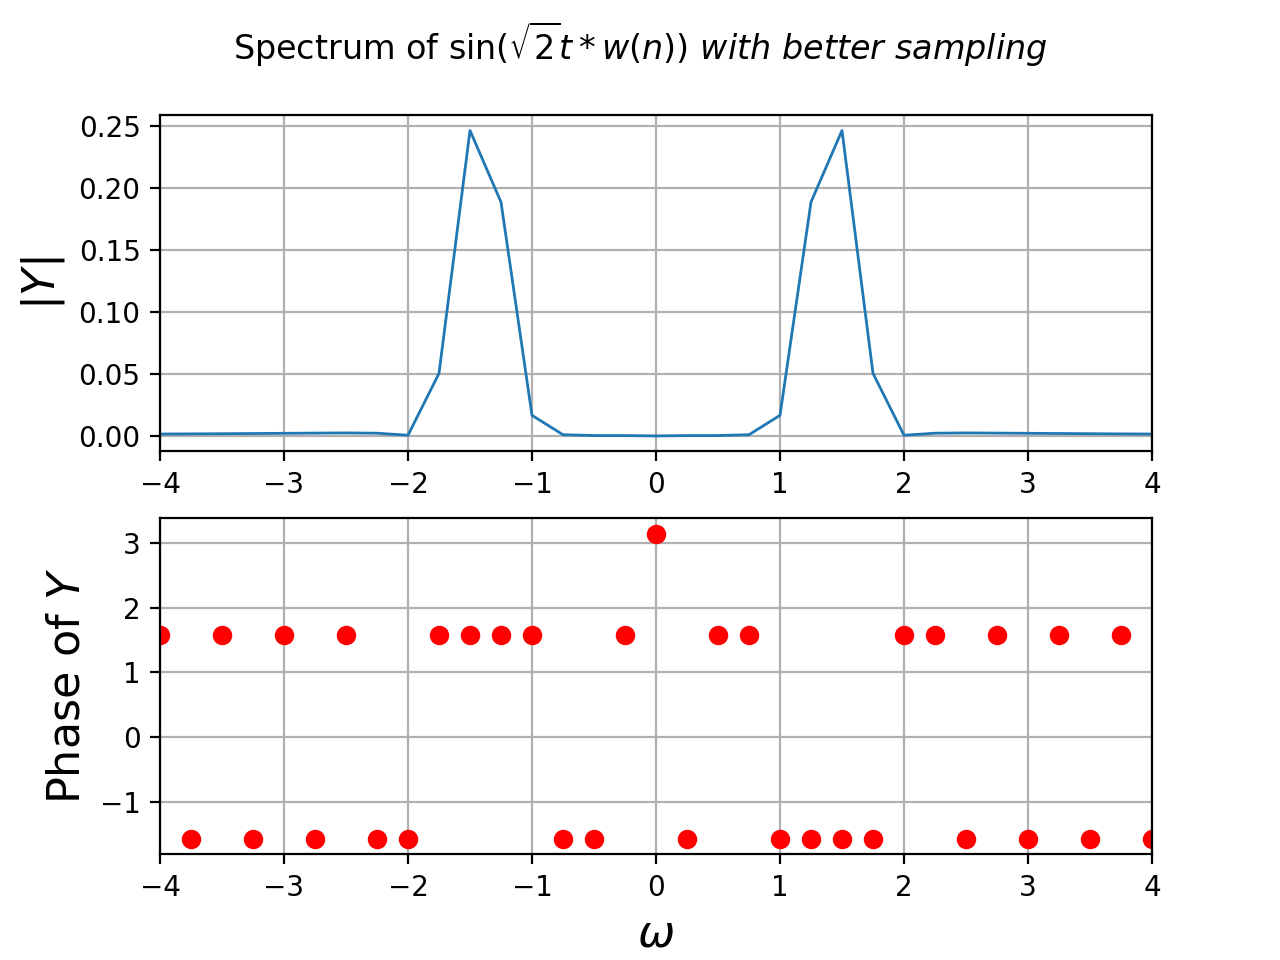
\includegraphics[scale=0.8]{ex_1_f4.png}
   	\label{fig:ex_1_f4}
   	\caption{Spectrum of $\sin(\sqrt{2} t)$ - obtained with 256 samples}
\end{figure}
{
We now obtain a good spectrum. But we still see two peaks, which is \textbf{not because of an approximation}, but it is the multiplication with hamming window that causes this broadening of peak. We can verify this by taking a different frequency of sinusoid like $\sin(1.25 t)$.
}


\subsection{QUESTION 2 - FFT of $\cos^3(\omega_{0} t)$} 
{
We find the spectrum of $\cos^3(\omega_{0} t)$ signal for $\omega_{0} = 0.86$, first without and then with windowing.
}
\begin{minted}{python3}
#Without windowing
y3 = lambda t: (cos(0.86*t))**3
ax1,ax2,*_ = DFT(y3,(-pi,pi),64,r'$\cos^{3}(\omega_{0}t)$')
ax1.set_xlim(-10,10)
ax2.set_xlim(-10,10)
show()

#With windowing
y3_w = lambda t: y3(t)*wnd(arange(256))
ax1,ax2,*_ = DFT(y3_w,(-4*pi,4*pi),256,r'$cos^{3}(\omega_{0}t)$')
ax1.set_xlim(-10,10)
ax2.set_xlim(-10,10)
show()
\end{minted}

\begin{figure}[H]
   	\centering
   	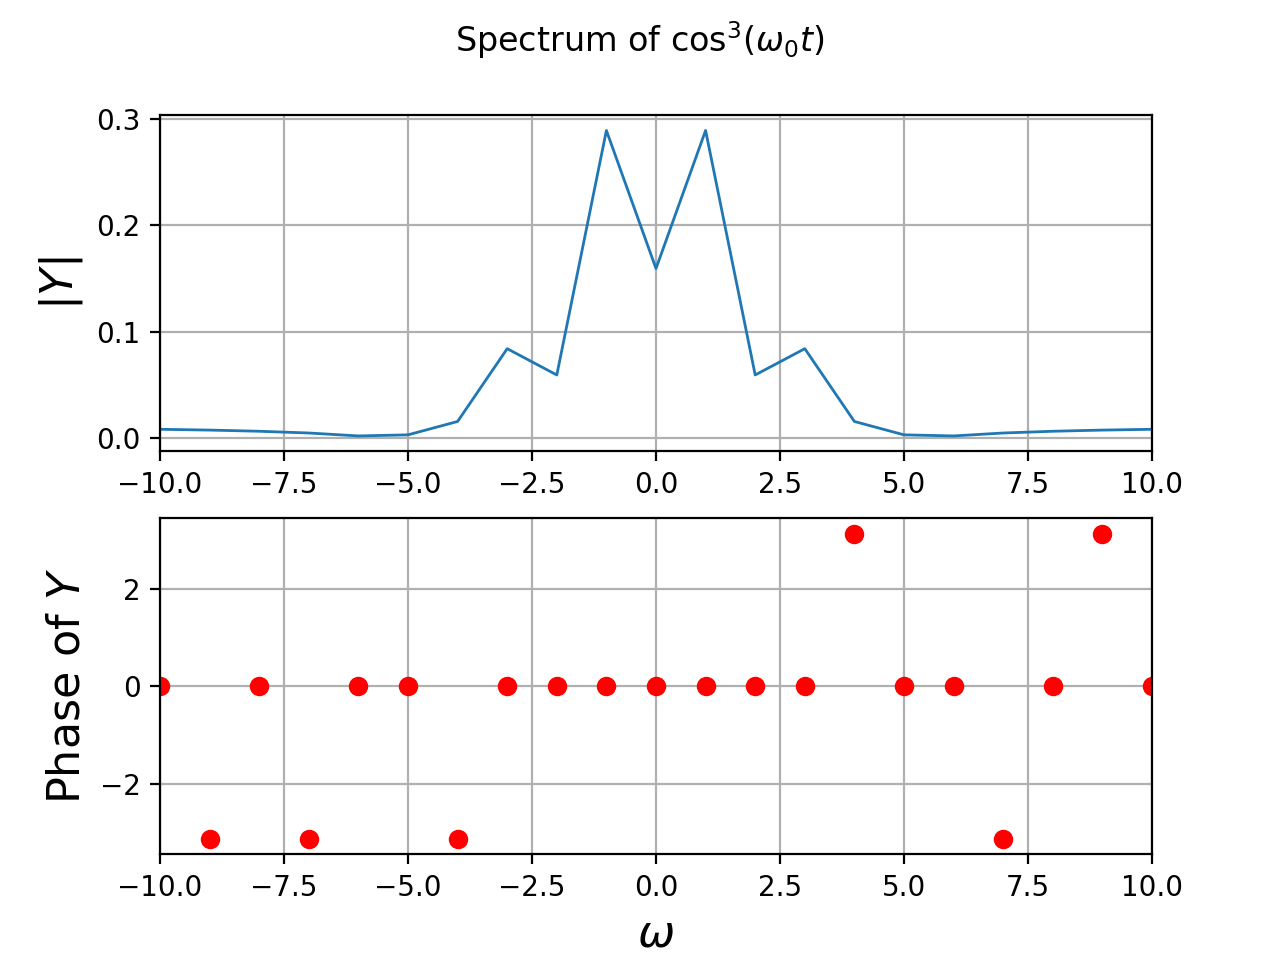
\includegraphics[scale=0.8]{qn2_wo.png}
   	\label{fig:qn2_wo}
   	\caption{Spectrum of $\cos^3(0.86 t)$ without windowing}
\end{figure}
\begin{figure}[H]
   	\centering
   	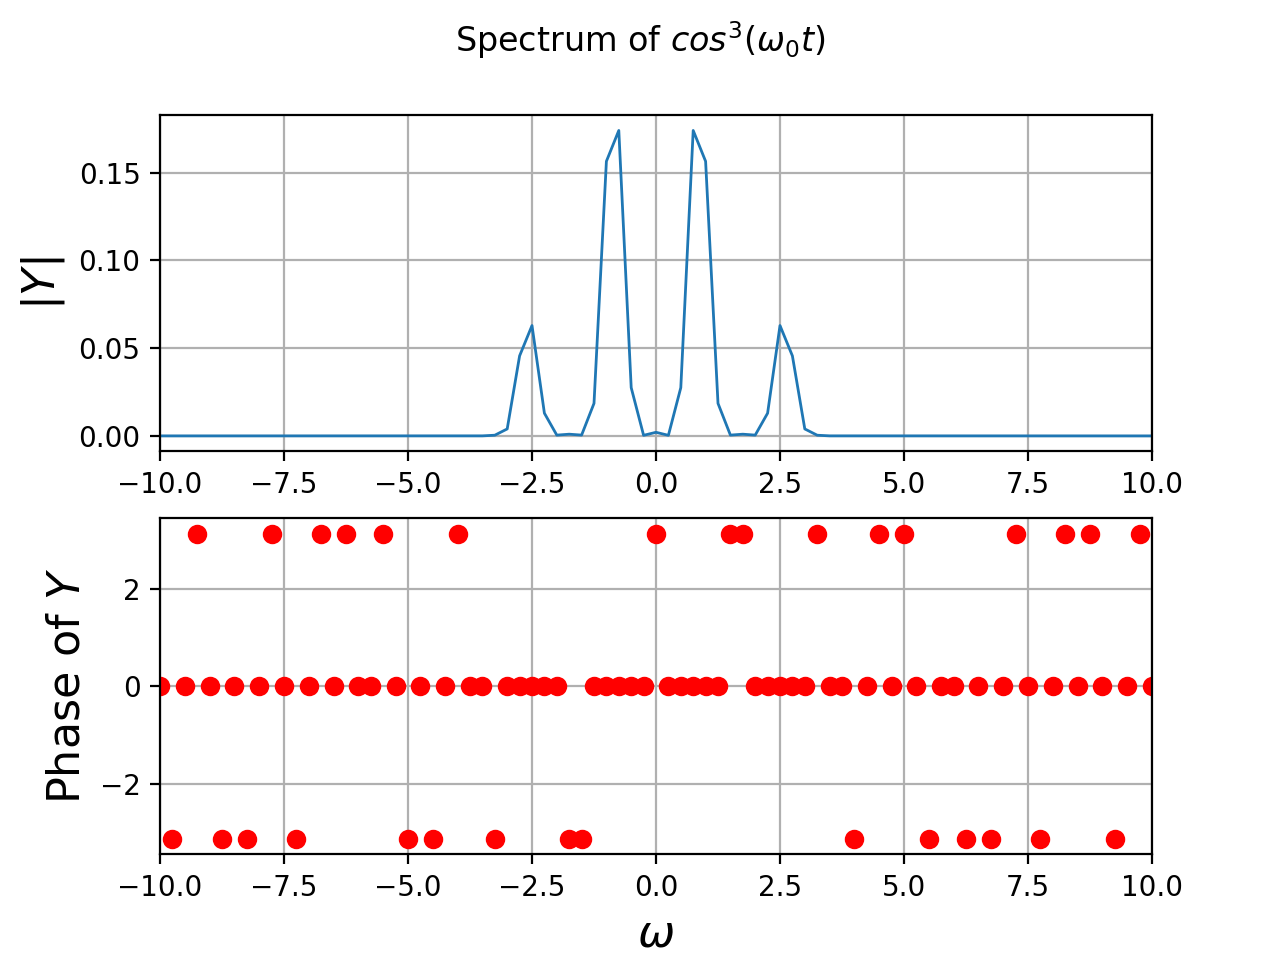
\includegraphics[scale=0.8]{qn2_wnd.png}
   	\label{fig:qn2_wnd}
   	\caption{Spectrum of $\cos^3(0.86 t)$ with windowing}
\end{figure}
{
We can clearly observe the role played by the hamming window in making the spectrum better by the \textbf{decaying the peaks faster} and make them look sharp.
}


\subsection{QUESTIONS 3,4 - FFT of $\cos(\omega_{0} t + \delta)$}
{
We plot the spectrum of $\cos(\omega_{0} t + \delta)$ without and with added Gaussian noise of amplitude 0.1 generate by randn() function in python. We sample 128 samples in $[-\pi,\pi)$ for obtaining the spectrum. We estimate the $\omega_{0}$ and $\delta$ from the spectrum obtained in both cases.
In both cases we have windowed the original function, which is $\cos(1.5 t + 0.5)$.
}
\begin{minted}{python3}
def est_delta(w,Y,sup = 1e-3,window = 1):
	'''Estimates delta (d) from the spectrum of cos(w*t+d)'''
	ii_1 = where(logical_and(abs(Y)>sup, w>0))[0]
	sort(ii_1)
	points = ii_1[1:window+1]
	#weighted average for first 2 points
	return sum(angle(Y[points]))/len(points)

def est_omega(w,Y):
	'''Estimates omega (w) from the spectrum of cos(w*t+d)'''
	ii = where(w > 0)
	#omega estimated by weighted average
	return sum(abs(Y[ii])**2 * w[ii])/sum(abs(Y[ii])**2)

def CosEst(ww,d):
    fn = lambda t:  cos(ww*t+d)*wnd(arange(len(t)))
    ax1,ax2,Y,w = DFT(fn,(-pi,pi),128,r'$cos(\omega_{0}t+\delta)$')
    ax1.set_xlim(-10,10)
    ax2.set_xlim(-10,10)
    show()

    print('Noiseless Signal parameters : ')
    print('\u03C9 :',est_omega(w,Y))
    print('\u03B4 :',est_delta(w,Y))
    return(Y)

Yf = CosEst(1.5,0.5)

def CosEst_Noisy(ww,d):
    fn = lambda t:  cos(ww*t+d)*wnd(arange(len(t))) + 0.1*randn(len(t))
    ax1,ax2,Y,w = DFT(fn,(-pi,pi),128,r'$cos(\omega_{0}t+\delta)\ with\ noise$')
    ax1.set_xlim(-10,10)
    ax2.set_xlim(-10,10)
    
    print('Noisy Signal parameters : ')
    print('\u03C9 :',est_omega(w,Y))
    print('\u03B4 :',est_delta(w,Y))
    return(Y)

Yf = CosEst_Noisy(1.5,0.5)
show()
\end{minted}

\begin{figure}[H]
   	\centering
   	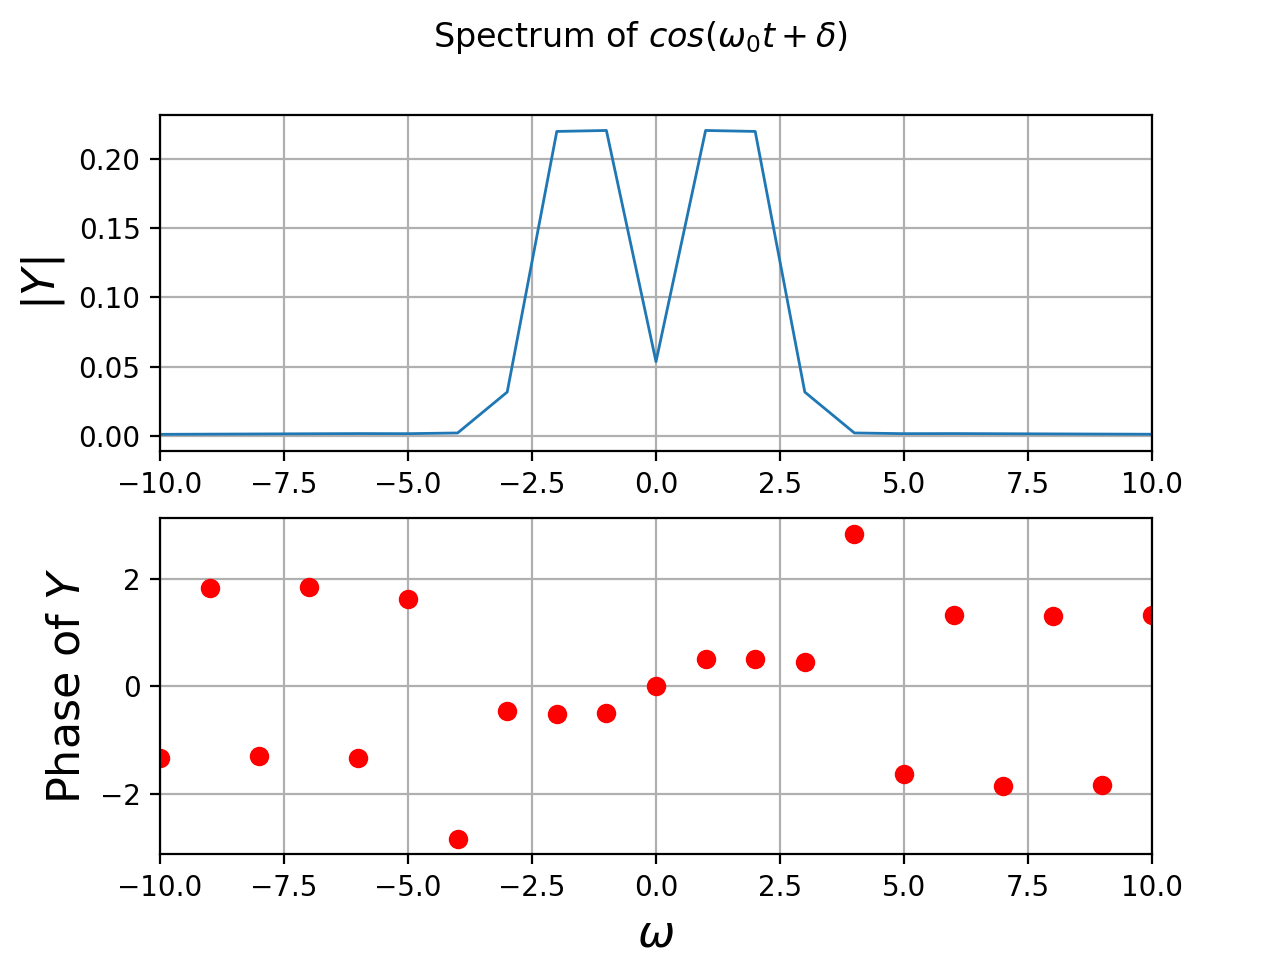
\includegraphics[scale=0.8]{qn4_wn.png}
   	\label{fig:qn4_wn}
   	\caption{Spectrum of $\cos(\omega_{0} t + \delta)$ without noise added}
\end{figure}
\begin{figure}[H]
   	\centering
   	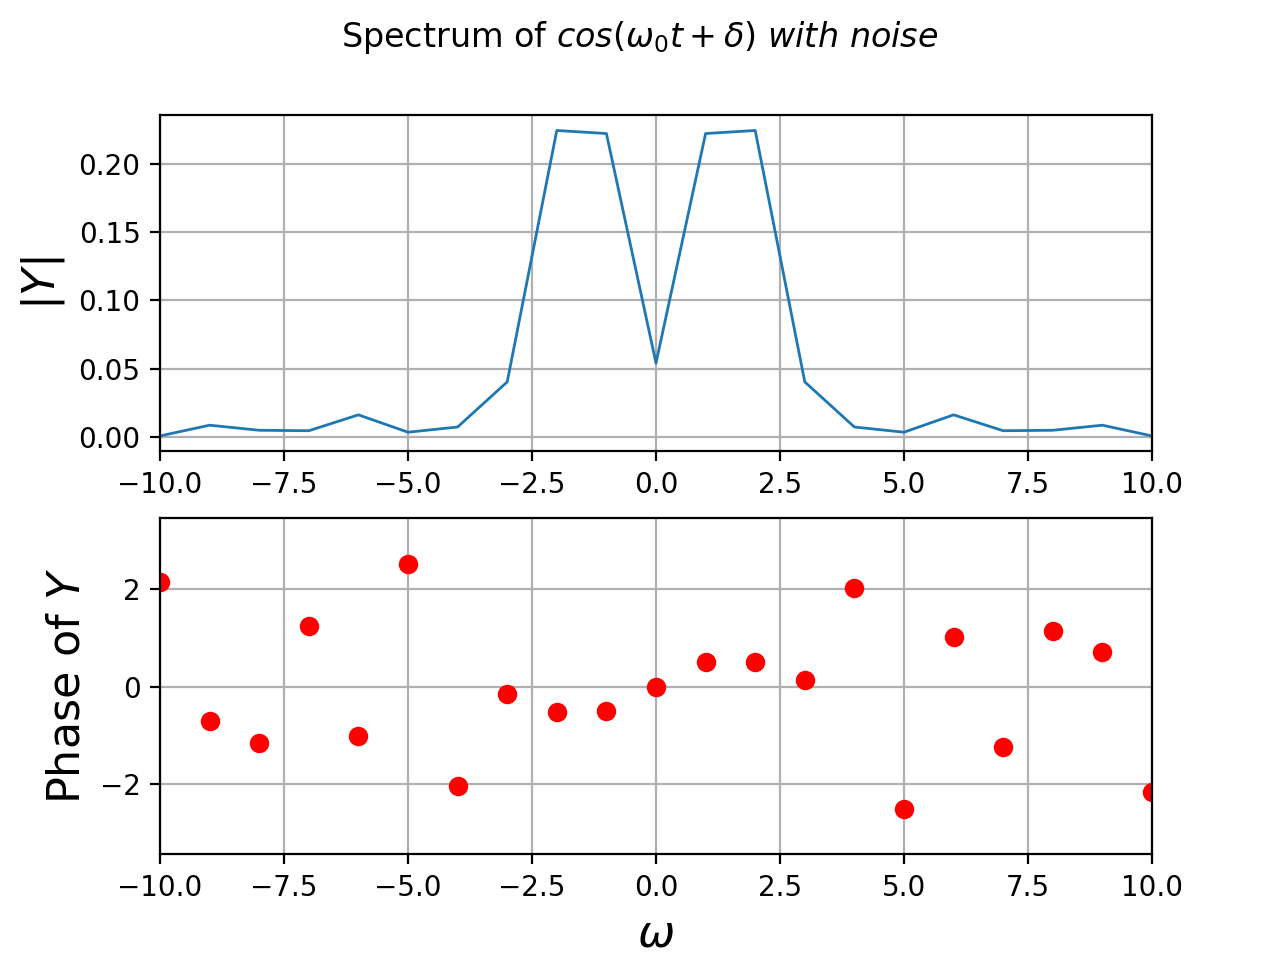
\includegraphics[scale=0.8]{qn4_n.png}
   	\label{fig:qn4_n}
   	\caption{Spectrum of $\cos(\omega_{0} t + \delta)$ with noise added}
\end{figure}
\begin{figure}[H]
   	\centering
   	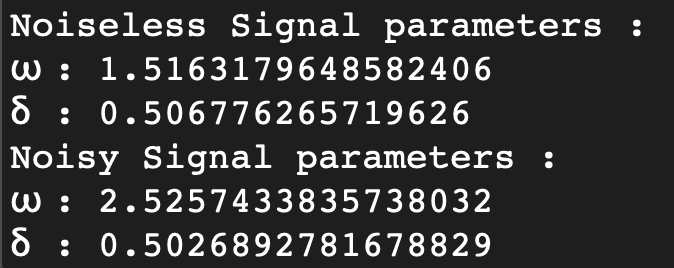
\includegraphics[scale=0.6]{out.png}
   	\label{fig:out}
   	\caption{Output of program estimating $\omega_{0}$ and $\delta$ for both cases}
\end{figure}
{
We can observe how our estimation strategies for obtaining $\omega_{0}$ and $\delta$ give close to accurate results. Noise is usually \textbf{high frequency component}, and we can also see how it affects our estimate of $\omega_{0}$.
}


\subsection{QUESTION 5 - FFT for Chirped Signal}
{
We obtain the DFT spectrum of the \textbf{chirped signal} - $\cos(16(1.5 + \frac{t}{2\pi})t)$ which is multiplied by the hamming window function.
\\We plot both the chirped signal alone in time domain and it's windowed version's DFT spectrum.
}
\begin{minted}{python3}
#Plotting the time domain signal
ychirp = lambda t: cos(16*t*(1.5+t/(2*pi)))*wnd(arange(len(t)))
figure()
t = linspace(-pi,pi,1024)
plot(t,ychirp(t))
xlabel('t')
ylabel('y(t)')
title("Chirped Signal in time domain")
show()

#Plotting the DFT spectrum
ax1,ax2,*_ = DFT(ychirp,(-pi,pi),1024,r'chirped signal')
ax1.set_xlim(-60,60)
ax2.set_xlim(-60,60)
show()
\end{minted}

\begin{figure}[H]
   	\centering
   	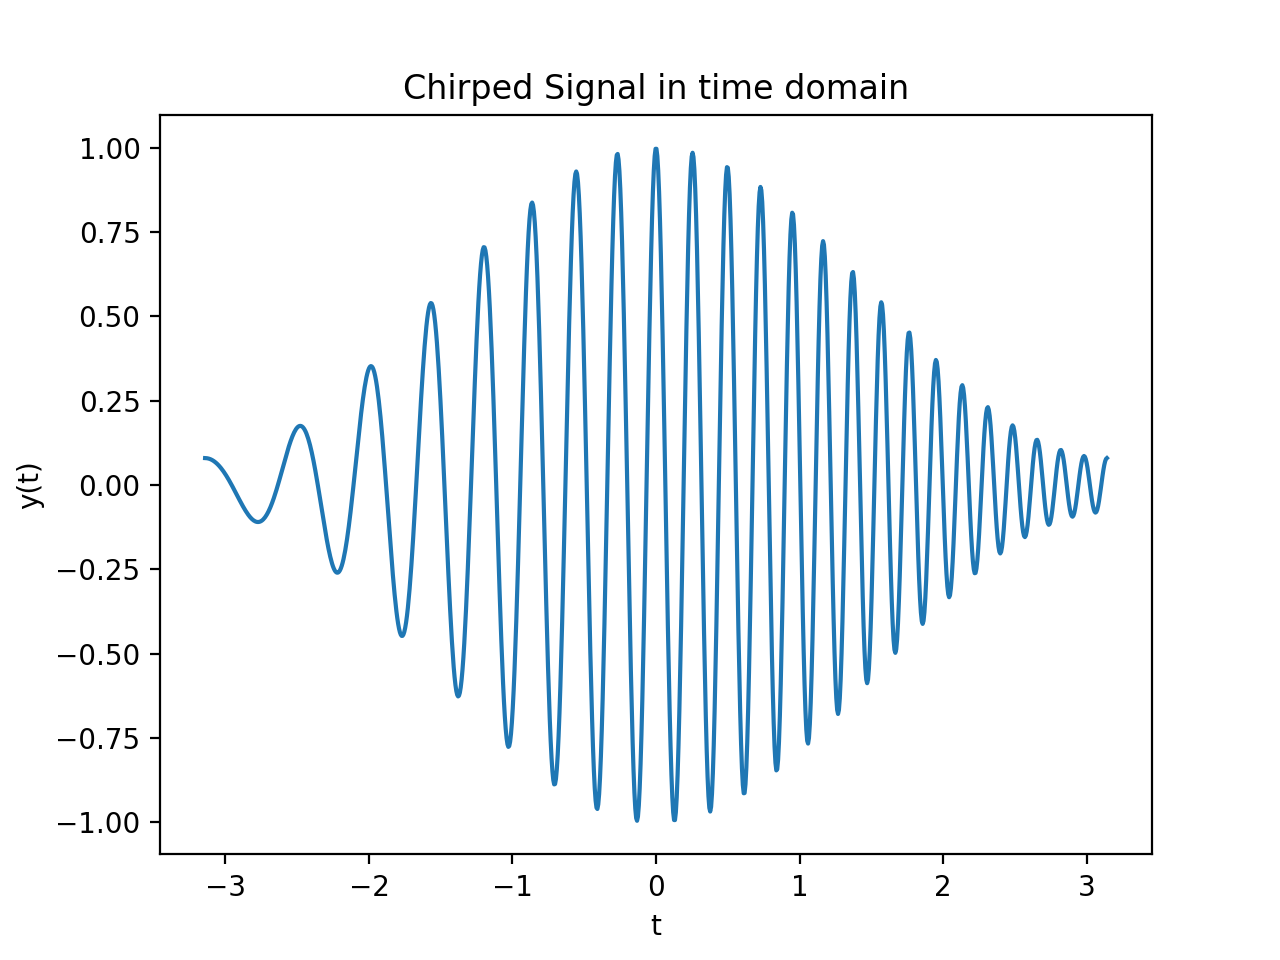
\includegraphics[scale=0.5]{qn5_t.png}
   	\label{fig:qn5_t}
   	\caption{Chirped signal in time domain}
\end{figure}
\begin{figure}[H]
   	\centering
   	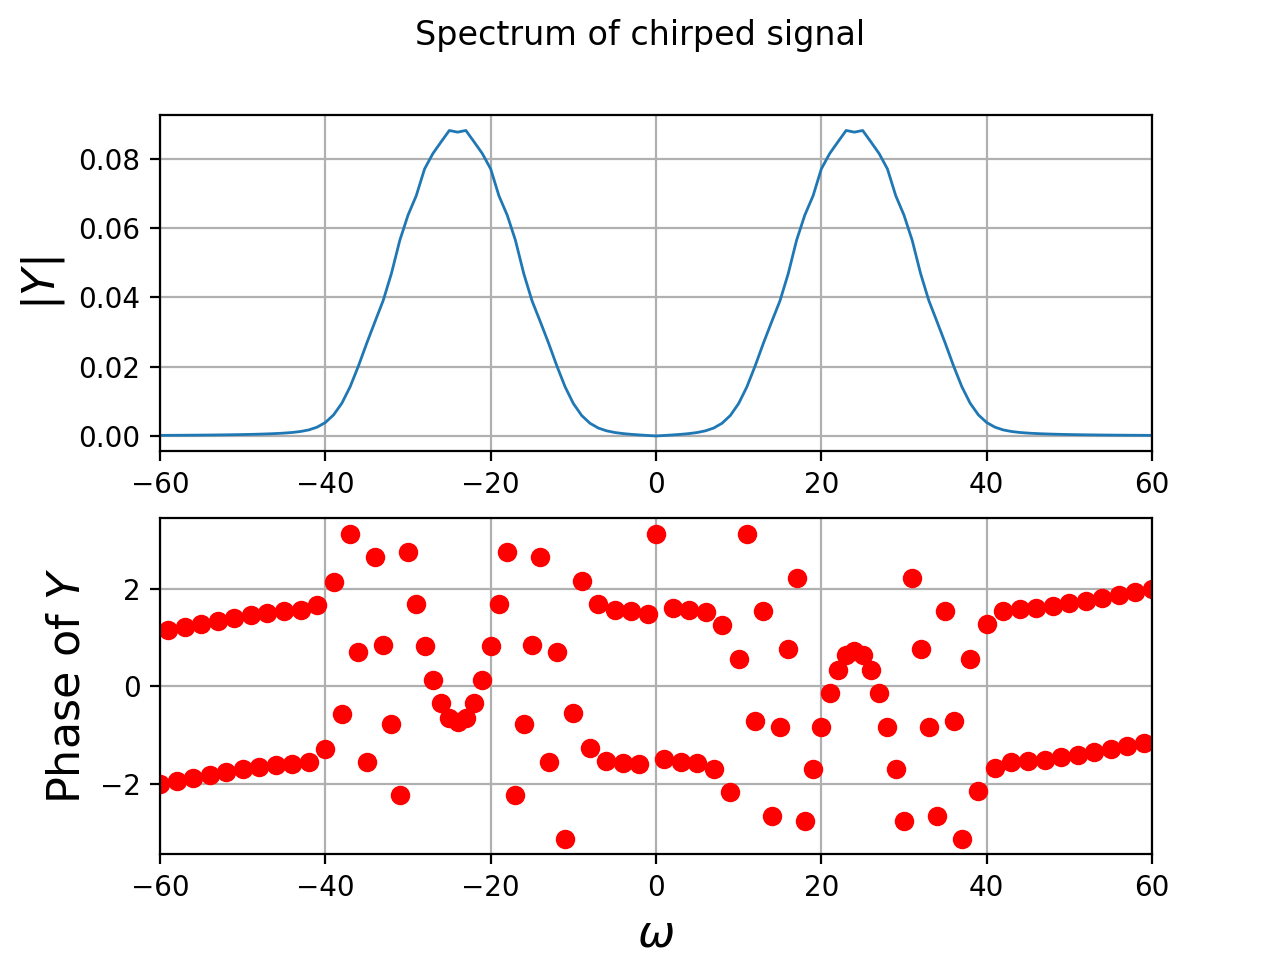
\includegraphics[scale=0.8]{qn5_spec.png}
   	\label{fig:qn5_spec}
   	\caption{DFT spectrum of chirped signal}
\end{figure}
{
We can notice how the frequency of the chirped signal increases as we go right in time from the time domain plot. We can also observe that the chirped signal has frequencies ranging from 16 to 32.
}


\subsection{QUESTION 6 - Time-Frequency plot of FFT for Chirped Signal}
{
Since the frequency of the chirped signal varies with time, we break the signal into various time intervals, window signal of each part separately, take their FFTs and plot their magnitude and phase in a 3-D spectrogram showing localized DFTs and evolution of the DFT spectrum with time.
\\We also make a contour plot of the magnitude to show them more clearly.
}
\begin{minted}{python3}
y_ch = cos(16*t*(1.5+t/(2*pi)))
NR = 64
NC = 1024//64
y_2D = zeros((NR,NC))
Y_2D = zeros((NR,NC),dtype = complex)
for i in range(NC):
	#Windowing
	y_2D[:,i] = y_ch[i*NR:(i+1)*NR]*wnd(arange(64))
	#The sample corresponding to -tmax should be set zero
	y_2D[0,i] = 0
	Y_2D[:,i] = fftshift(fft(fftshift(y_2D[:,i])))/float(NR)
x = linspace(-pi,pi,16,endpoint = False)
w = linspace(-pi,pi,64,endpoint = False)
w = w*1024.0/(2*pi);
#Forming the x and y values for the surface plot
wv,xv = meshgrid(w,x,indexing = 'ij')

#We plot the surface plot of magnitude of Y
fig = figure()
ax = p3.Axes3D(fig)
title('3-D spectrogram - Magnitude')
surf = ax.plot_surface(wv,xv,abs(Y_2D),cmap = cm.coolwarm,linewidth = 0,
			antialiased = False)
fig.colorbar(surf,shrink = 0.5,aspect = 5)
xlabel("Frequency")
ylabel("Time")
show()

#We plot the contour plot of magnitude of Y
fig = figure()
title('Contour plot of Magnitude')
surf = contourf(xv,wv,abs(Y_2D))
ylim([-50,50])
ylabel("Frequency")
xlabel("Time")
fig.colorbar(surf)
show()

#We plot the surface plot of angle of Y
fig = figure()
ax = p3.Axes3D(fig)
title('3-D spectrogram - Angle')
surf = ax.plot_surface(wv,xv,angle(Y_2D),cmap = cm.coolwarm,linewidth = 0,
			antialiased = False)
fig.colorbar(surf,shrink = 0.5,aspect = 5)
xlabel("Frequency")
ylabel("Time")
show()
\end{minted}

\begin{figure}[H]
   	\centering
   	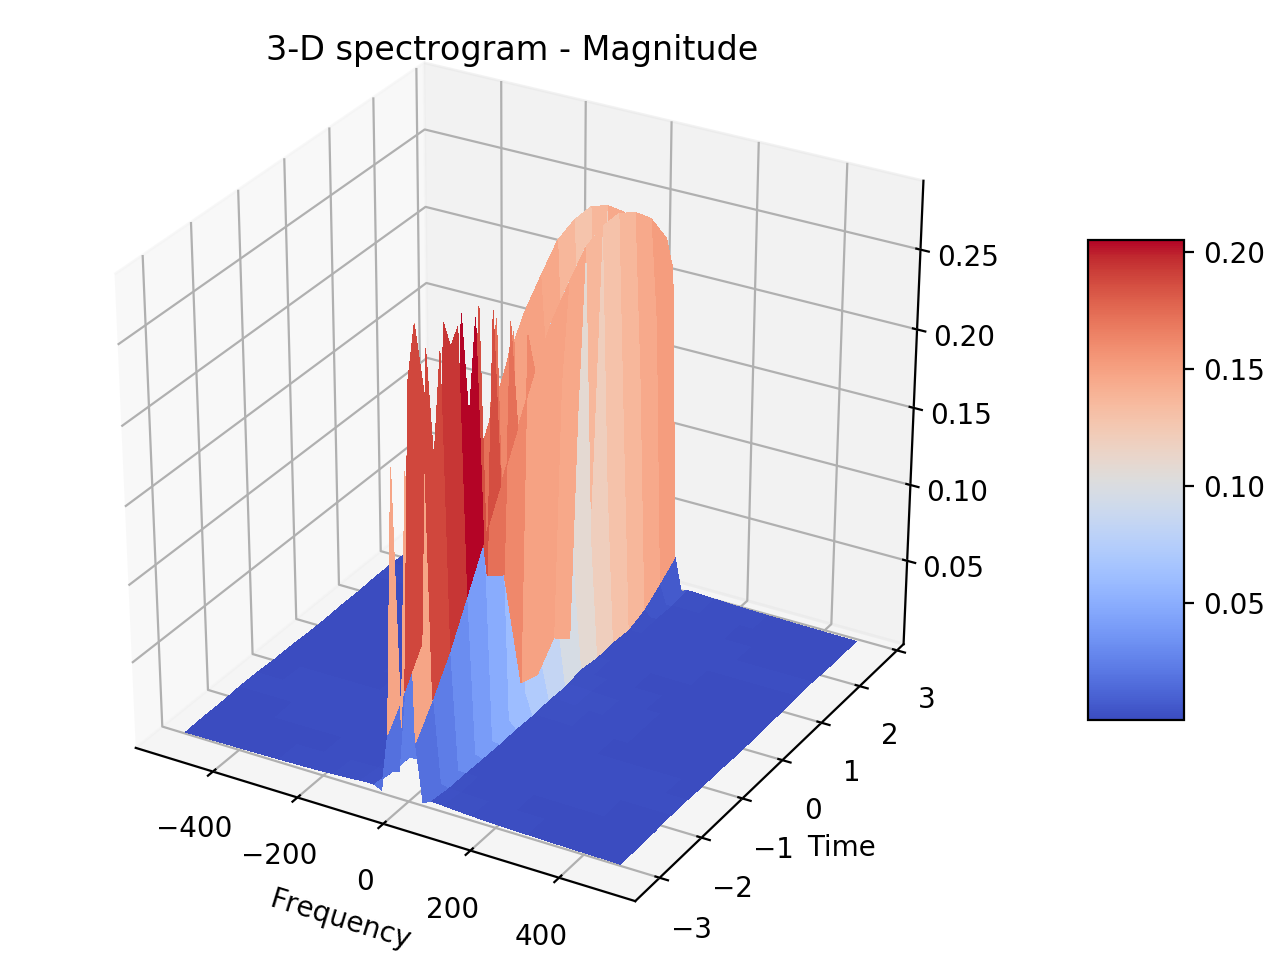
\includegraphics[scale=0.5]{qn6_mag.png}
   	\label{fig:qn6_mag}
   	\caption{3-D spectrogram depicting Magnitude of localized DFTs}
\end{figure}
\begin{figure}[H]
   	\centering
   	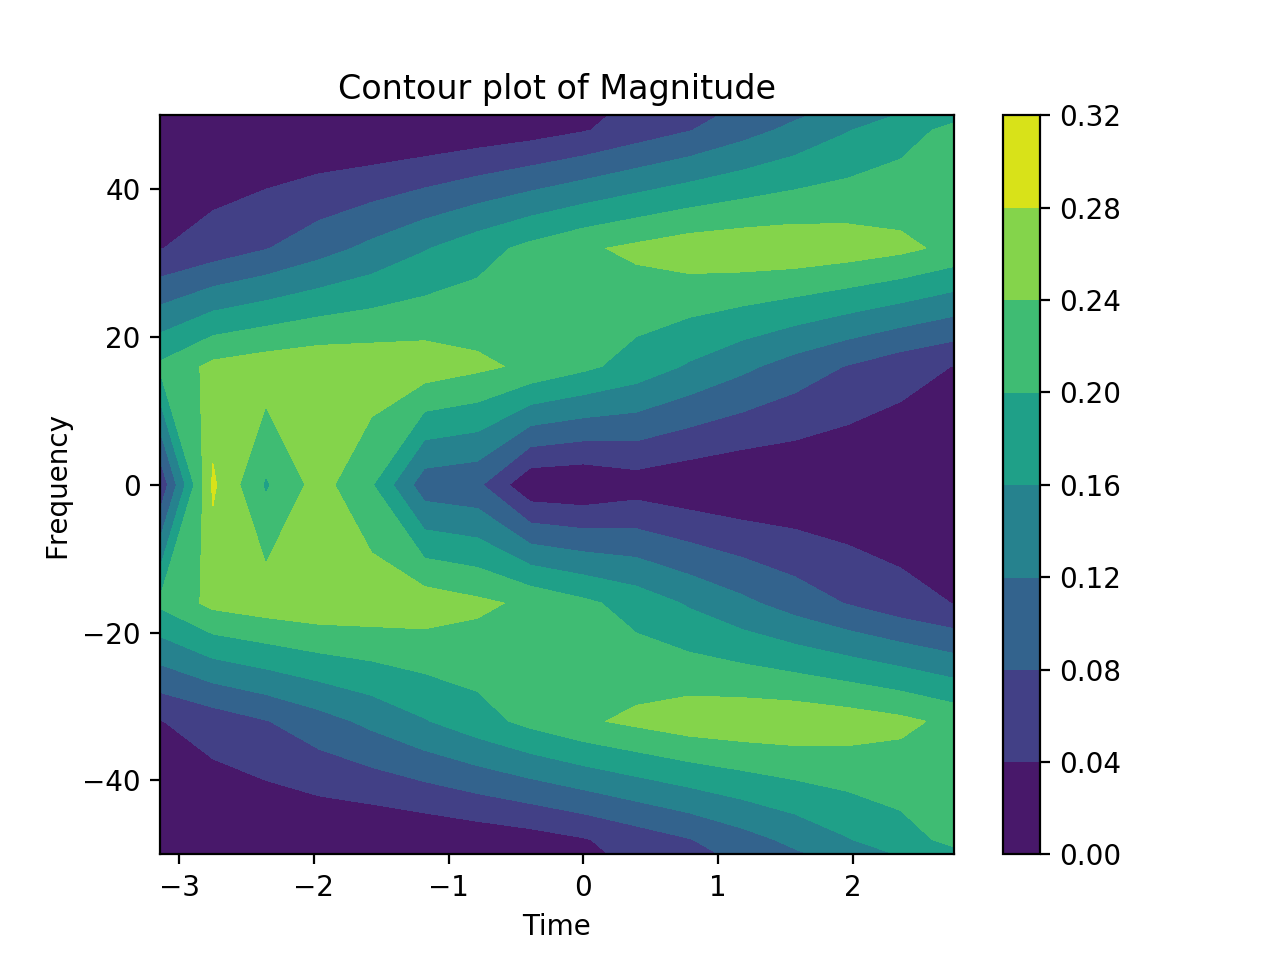
\includegraphics[scale=0.5]{qn6_cont.png}
   	\label{fig:qn6_cont}
   	\caption{Contour plot depicting Magnitude of localized DFTs}
\end{figure}
\begin{figure}[H]
   	\centering
   	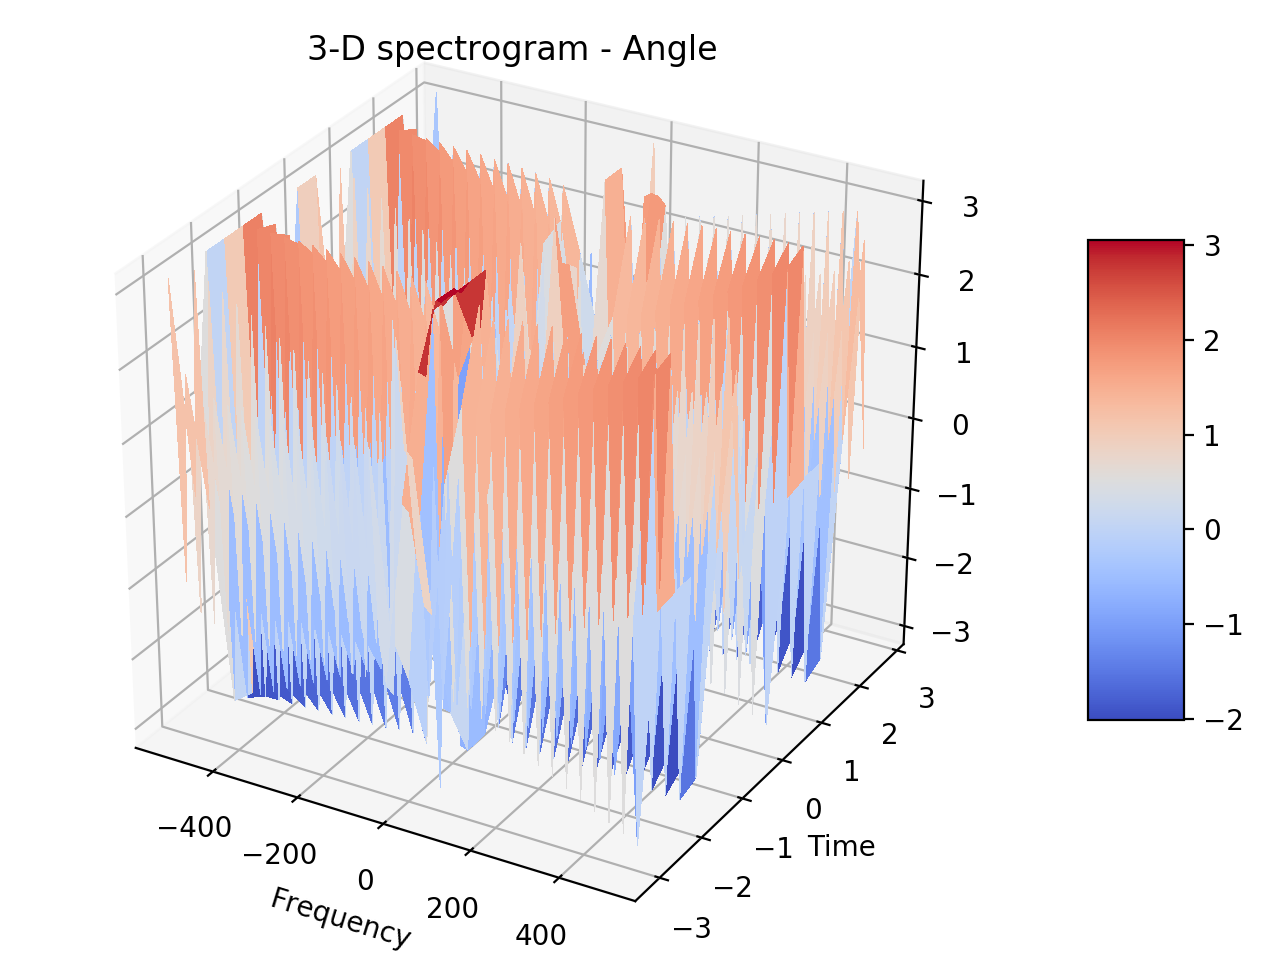
\includegraphics[scale=0.5]{qn6_ang.png}
   	\label{fig:qn6_ang}
   	\caption{3-D spectrogram depicting Phase of localized DFTs}
\end{figure}
{
From the contour plot of the magnitude, it's clear how the frequency changes from 16 to 32 as time evolves.
}


\section{Conclusions}
\begin{itemize}
\item We obtained the DFT of non-periodic signals, analysed and made them better.
\item We understood the usage of windowing functions (like Hamming Window we used in this assignment) in improving the spectrum of non-periodic signals.
\item We analysed the chirped signal in time domain, frequency domain and also by plotting the Time-Frequency plot.
\end{itemize}

\end{document}